%; whizzy chapter
% -initex iniptex -latex platex -format platex -bibtex jbibtex -fmt fmt
% 以上 whizzytex を使用する場合の設定。

%     Kansai Debian Meeting resources
%     Copyright (C) 2007 Takaya Yamashita
%     Thank you for Tokyo Debian Meeting resources

%     This program is free software; you can redistribute it and/or modify
%     it under the terms of the GNU General Public License as published by
%     the Free Software Foundation; either version 2 of the License, or
%     (at your option) any later version.

%     This program is distributed in the hope that it will be useful,
%     but WITHOUT ANY WARRANTY; without even the implied warranty of
%     MERCHANTABILITY or FITNESS FOR A PARTICULAR PURPOSE.  See the
%     GNU General Public License for more details.

%     You should have received a copy of the GNU General Public License
%     along with this program; if not, write to the Free Software
%     Foundation, Inc., 51 Franklin St, Fifth Floor, Boston, MA  02110-1301 USA

%  preview (shell-command (concat "evince " (replace-regexp-in-string "tex$" "pdf"(buffer-file-name)) "&"))
% 画像ファイルを処理するためにはebbを利用してboundingboxを作成。
%(shell-command "cd image200708; ebb *.png")

%%ここからヘッダ開始。

\documentclass[mingoth,a4paper]{jsarticle}
\usepackage{kansaimonthlyreport}
\usepackage{ulem}
\usepackage{enumitem}

% 日付を定義する、毎月変わります。
\newcommand{\debmtgyear}{2019}
\newcommand{\debmtgdate}{22}
\newcommand{\debmtgmonth}{12}
\newcommand{\debmtgnumber}{153}

\def\fixme#1{{\color{red}{#1}}}

\begin{document}

\begin{titlepage}

% 毎月変更する部分、本文の末尾も修正することをわすれずに

 第\debmtgnumber{}回 関西 Debian 勉強会資料

\vspace{2cm}

\begin{center}
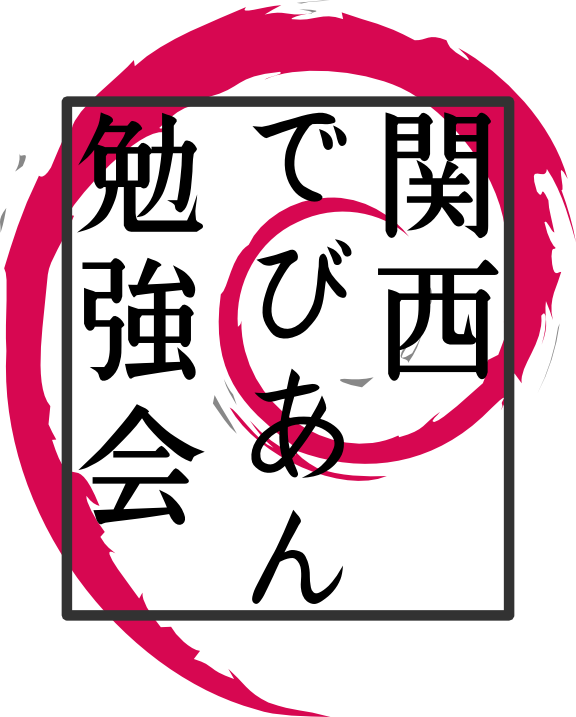
\includegraphics[width=.99\linewidth,clip]{image200802/kansaidebianlogo.png}
\end{center}

\begin{flushright}
\hfill{}関西 Debian 勉強会担当者 佐々木・倉敷・のがた・かわだ・おおつき \\
\hfill{}\debmtgyear{}年\debmtgmonth{}月\debmtgdate{}日
\end{flushright}

\thispagestyle{empty}
\end{titlepage}

\dancersection{最近のDebian関係のイベント報告}{Debian JP}

\dancersection{事前課題}{関西Debian勉強会}

参加者の皆さんは以下の通りです:
\begin{prework}{}
\end{prework}

\dancersection{Debian パッケージ作成入門2019}{佐々木洋平}

\vspace*{-2em}
\subsection{はじめに}

お題を「Debianパッケージ作成入門2019」としていますが、
最初からやっていたら流石に時間が足りません。
%
モダンなDebianパッケージ作成に関するチュートリアルとしては、
本勉強会リポジトリ内の文書群に加え、
Lucas, N., 2019: ``Debian Packaging Tutorial'' (倉沢望 訳: 「Debianパッケージングチュートリアル」)\footnote{%
  下記の URL に PDF 版が公開されています。
  \begin{itemize}[itemsep=0pt,topsep=0pt]
  \item %
    \url{https://www.debian.org/doc/manuals/packaging-tutorial/packaging-tutorial.en.pdf}
  \item %
    \url{https://www.debian.org/doc/manuals/packaging-tutorial/packaging-tutorial.ja.pdf}
  \end{itemize}
}が非常に参考になるでしょう。
なお、
この文書は\texttt{packaging-tutorial}としてDebianパッケージにもなっていますので
\begin{commandline}
  % sudo apt install packaging-tutorial
\end{commandline}
として眺められるようにしておくと良いかもしれません。
%
今回の発表では、
この文書に触れられていなかった最近の話題の幾つかについて簡単にまとめてみようと思います\footnote{%
  そういう意味では, 「パッケージ作成入門」はタイトルに偽りあり, ですねぇ$\cdots$%
}。
なお、Debian Policyの方はガシガシと更新されていますので、こちらを参照されるのが良いでしょう。

\subsection{\texttt{Build-Depends:debhelper-compat}}

\texttt{debian/compat}ファイルはdebhelperの互換性レベルを規定するファイルで、
後方互換性を保持するために使われます。ファイルの中身は、たいていバージョン番号が記載された行のみからなります。
\begin{commandline}
  例: アップグレード前の howm の debian/compat
  % cat debian/compat
  11
\end{commandline}
\noindent
実の所、\texttt{debian/control}の中身にも
\begin{commandline}
  Build-Depends: debhelper (>= 11~), ...
\end{commandline}
\noindent
という行があるので、情報が重複していますね。
%
\texttt{debhelper >= 12}より、これらをスッキリと整理した書き方が可能になっています。
\begin{commandline}
  % cat debian/control
  ...
  Build-Depends: debhelper-compat (=12), ...
  ...
  % rm debian/compat   # ← 不要だ!
\end{commandline}

\subsection{\texttt{Rules-Requires-Root}}

lintian さんに怒られて気がついたのですが、\texttt{debian/control}内に新しく
\textbf{Rules-Requires-Root}というフィールドが増えていました。
Debian Policy内では
\begin{quote}
  Simple field that defines if the source package requires access to
  root (or fakeroot) during selected targets in the Main building
  script: debian/rules.
\end{quote}
とされています。

佐々木がメンテしているパッケージでは、今のところ\texttt{debian/rules}での処理において
\texttt{root} (or \texttt{fakeroot})が必要となる状況はありませんが、
必要に応じてこれを明示的に指定する必要があります%
\footnote{%
  勉強会当日も、あーでもないこーでもない、と話が紛糾.
  例として、谷口さんの \texttt{xgalaga++} での紹介がありました。
  \\
  \@see \texttt{https://salsa.debian.org/games-team/xgalagapp}
}。

\subsection{salsaでCI}

佐々木は ruby-team に所属しています。
最近、salsaのruby-teamのリポジトリ全てに\texttt{debian/salsa-ci.yml}が
コミットされました
\footnote{%
  アナウンス\sout{無くて}気がつかなくてビビった。
  どうも IRC と debconf では会話があった模様。
}。
例として、\texttt{rabbit}の\texttt{debian/salsa-ci.yml}を眺めてみると
\begin{commandline}
---
include:
  - https://salsa.debian.org/salsa-ci-team/pipeline/raw/master/salsa-ci.yml
  - https://salsa.debian.org/salsa-ci-team/pipeline/raw/master/pipeline-jobs.yml

variables:
  SALSA_CI_DISABLE_BLHC: 1
  SALSA_CI_DISABLE_BUILD_PACKAGE_ANY: 1
\end{commandline}
\noindent
となっています。安直には、上の二つのYAMLファイルをincludeすれば、
一通りのパッケージテストが定義されることになるでしょう。
詳細は
\begin{center}
  \texttt{https://salsa.debian.org/salsa-ci-team/pipeline}
\end{center}
を参照して下さい。
なお、これをパッケージディレクトリに放り込んだだけでCIが走るわけではありません。
salsaの側で、pipeline を有効化しておくのを忘れない様にしておきましょう。
\begin{figure}[htbp!]
  \centering
  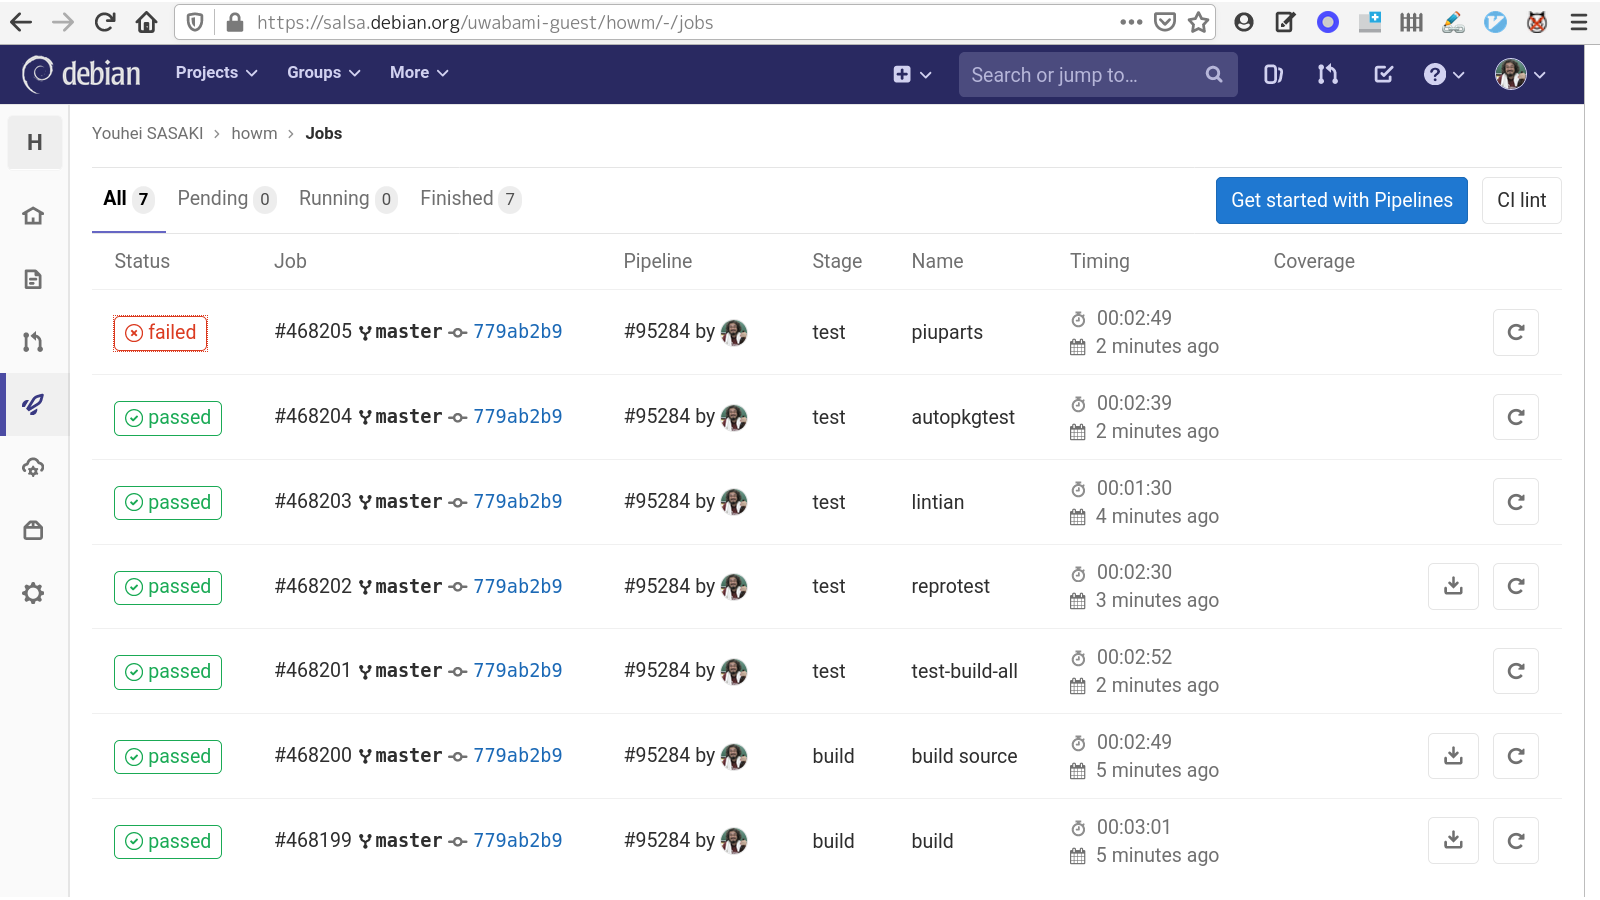
\includegraphics[height=.26\textheight]{image201912/2019-12-22-salsa-ci.png}
  \caption{salsaでのCIの結果(おや, 一番上のpipelineの様子が...)}
\end{figure}

現場からは以上です。\hfill(勉強会ご参加の皆様、ありがとうございました)

\clearpage

\dancersection{開催の予定}{}


\vspace{\fill}
本資料は GPL v 2.0 のライセンスで公開いたします。

\clearpage

%
% 冊子にするために、4の倍数にする必要がある。
% そのための調整

\mbox{}\newpage
\mbox{}\newpage

\printindex
%\cleartooddpage

 \begin{minipage}[b]{0.2\hsize}
  \rotatebox{90}{\fontsize{80}{80} {\gt 関西 Debian 勉強会} }
 \end{minipage}
 \begin{minipage}[b]{0.8\hsize}

 \vspace*{15cm}
 \rule{\hsize}{1mm}
 \vspace{2mm}
 
\includegraphics[width=2cm,clip]{image200502/openlogo-nd.eps}
 \noindent \Large \bfseries{Debian 勉強会資料}\\ \\
 \noindent \normalfont \debmtgyear{}年\debmtgmonth{}月\debmtgdate{}日 \hspace{5mm}  初版第1刷発行\\
 \noindent \normalfont 関西 Debian 勉強会 (編集・印刷・発行)\\
 \rule{\hsize}{1mm}
 \end{minipage}

\end{document}
